\begin{figure}[h!t]{\textwidth}
	\centering
    \caption{Slight difference between electricity sector concepts.} \label{fig:sector}
    
    \tikzstyle{arrow} = [thick,->,>=stealth, line width=1pt]
    \tikzstyle{drew} = [draw,fill=white,rounded corners=0.1cm]
    
    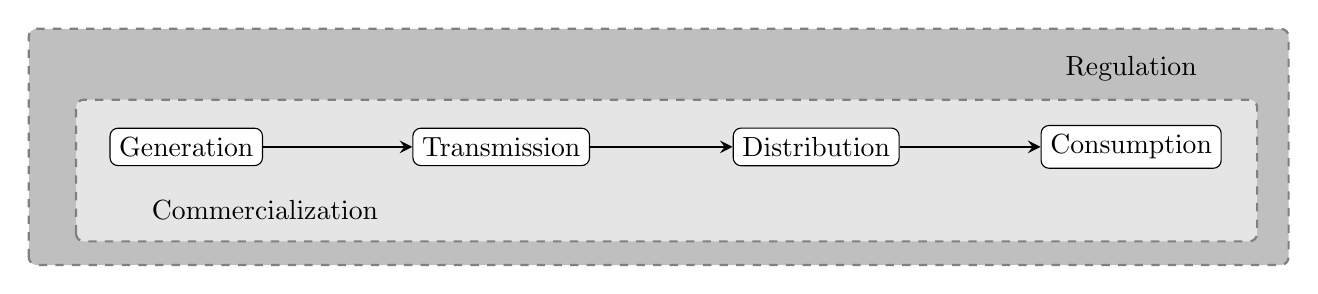
\begin{tikzpicture}
        % place dimensions
        \draw[gray,thick,dashed,fill=gray!50,rounded corners=0.1cm] (-2,-1.5) rectangle (14,1.5);
        \draw[gray,thick,dashed,fill=gray!20,rounded corners=0.1cm] (-1.4,-1.2) rectangle (13.6,0.6);
        
        % place nodes
        \node[drew] at (0, 0)		(g) {Generation};
        \node[drew] at (4, 0)		(t) {Transmission};
        \node[drew] at (8, 0)		(d) {Distribution};
		\node[drew] at (12, 0)		(c) {Consumption};
        \node		at (1, -0.8)	(o) {Commercialization};
        \node		at (12, 1)		(r) {Regulation};

        % draw connections
        \draw[arrow] (g) -- (t);
        \draw[arrow] (t) -- (d);
        \draw[arrow] (d) -- (c);
    \end{tikzpicture}
    
  	\legend{While electric power basic infrastructure is on white boxes,
    electricity sector pattern involves greater integrations as shown by gray boxes.
    The presence and relationships of agents on each segment is indicated as well.}
    \source{Author.}
\end{figure}